\documentclass[12pt,a4paper,fleqn]{article}
\title{Progress Report}
\author{Syed Ahmad Raza}
\date{2016.12.20}
\usepackage{mathtools}
\usepackage{graphicx}
\usepackage{color}          % for color eps output
%\usepackage{layouts}       % for: \printinunitsof{in}\prntlen{\textwidth}

\begin{document}
\maketitle
\section*{Numerical solution for 2D heat transfer}
A C++ code was written to solve the problem of 2D heat transfer. Forward in time
center in space (FTCS) method was used with the following formula:
\begin{equation}
T_i^{n+1} = T_i^n + \Delta t \alpha(\frac{\partial^2T}{\partial x^2} +
\frac{\partial^2T}{\partial y^2})
\end{equation}

A time step of 0.001 was utilized with 200 grid intervals in both x and y
directions. %Two sets of boundary conditions were considered.

Initial condition was $T_i=25^{\circ}C$.

Boundary conditions for the first case were selected as follows:
\begin{enumerate}
\item $T_{xi}=25^{\circ}C$ at $x=0$
\item $T_{xf}=25^{\circ}C$ at $x=L$
\item $T_{yi}=25^{\circ}C$ at $y=0$
\item $T_{yf}=50^{\circ}C$ at $y=L$
\end{enumerate}

\begin{figure}[p!]
\centering
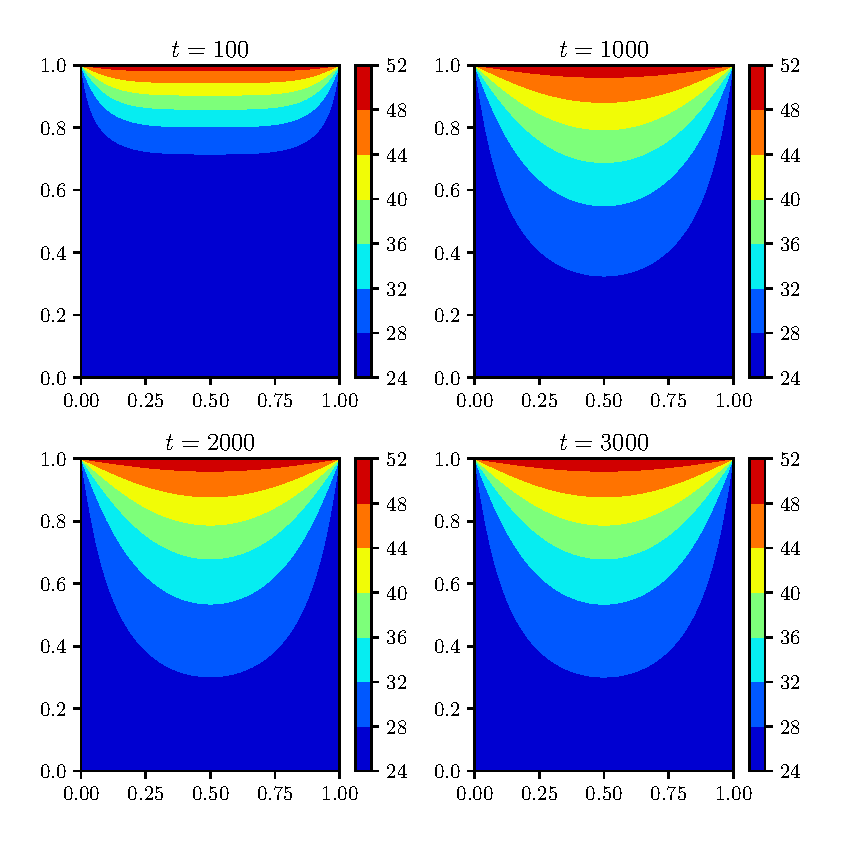
\includegraphics[width=\linewidth]{ht2dCase01.eps}
\caption{Plots for the first case with various values of time (time step of
0.001).}
\end{figure}

% \newpage
% Boundary conditions for the second case were selected as follows:
% \begin{enumerate}
% \item $T_{xi}=25^{\circ}C$ at $x=0$
% \item $T_{xf}=50^{\circ}C$ at $x=L$
% \item $T_{yi}=25^{\circ}C$ at $y=0$
% \item $T_{yf}=50^{\circ}C$ at $y=L$
% \end{enumerate}
% The initial condition was kept the same. However, steady state was not achieved
% for the test durations used.
% 
% \begin{figure}[p!]
% \centering
% 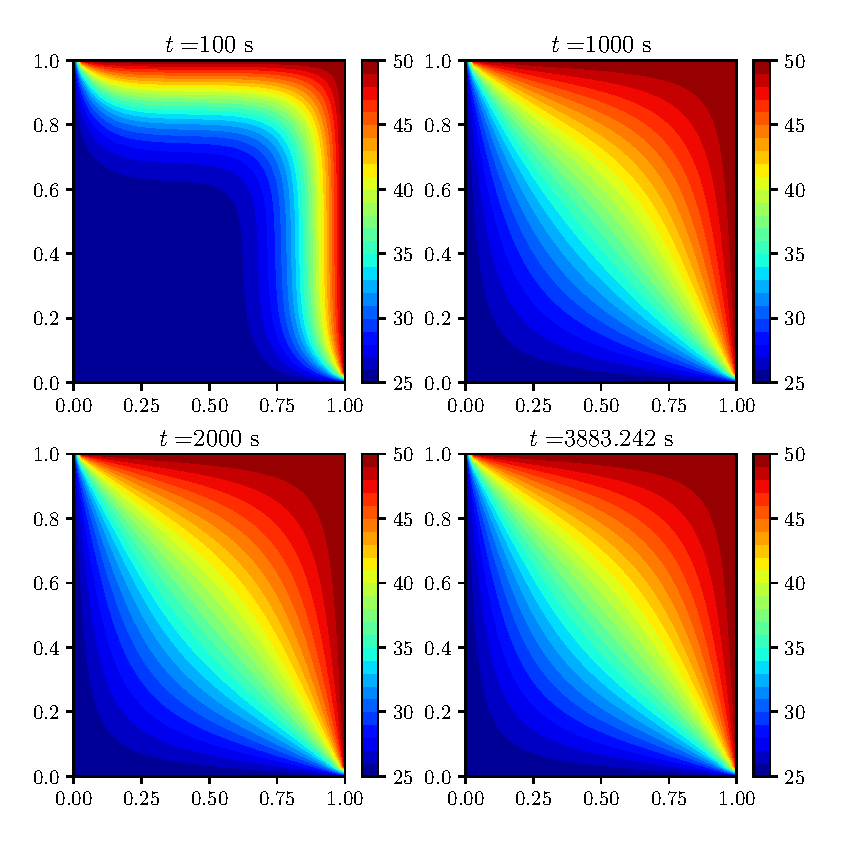
\includegraphics[width=\linewidth]{ht2dCase02.eps}
% \caption{Plots for the first case with various values of time (time step of
% 0.001).}
% \end{figure}
\end{document}
